This first chapter addresses the questions ``When should we trust a dynamics model?'' and  ``What do we do if the model is unreliable at the current state?''. I introduce a formal problem statement for planning with unreliable dynamics, and formalize learning reliability as a binary classification problem. I then propose methods for learning this classifier and using this classifier in planning. I also define what it means to be in need of recovery in terms of the classifier. Using this definition, I then propose a method for learning a recovery policy for these states using the data already collected for the classifier.

\section{Introduction} \label{SciRob:sec:intro}

Control and motion planning methods that rely on models to predict the outcomes of potential actions are ubiquitous in robotics. But whether these models are analytical, simulated, learned, or implicit within a policy, they are only as valid as the assumptions used to create them. When encountering a real-world unstructured environment, these assumptions may be violated, rendering a model unreliable \cite{Wang2019}. What is worse, estimating how erroneous our models are is difficult, as methods that predict uncertainty distributions based on training data \cite{Chua2018,Lakshminarayanan2017} don’t account for novel scenarios, e.g. when new types of constraints are introduced. This is especially problematic if these constraints are not easily represented \cite{Kamthe2018} in the model’s state space. Consequently, the inability to generate meaningful predictive uncertainty distributions for novel scenarios precludes the use of belief-space planning techniques \cite{WangBounded2018,FIRM,LQGMP}.

Roboticists rarely address the unreliable model problem directly; instead, we often resort to high-frequency re-planning, hoping to compensate for model errors online \cite{Finn2017,Koller2019}. But this kind of approach assumes that the erroneous model is somehow likely to produce useful short-horizon actions. While it may not be possible to create universally-valid models of complex high-degree-of-freedom systems such as deformable objects, this does not preclude using imperfect models to perform useful tasks. For example, we do not need to know all the friction and stiffness properties of a rope to drag it along the ground. The key questions, which have, until now, received very little attention, are \textit{1) When should we trust a model?} and \textit{2) What do we do if the robot is in a state where the model is unreliable?} Addressing these questions is paramount if we wish to deploy robots in unstructured environments such as homes and industrial sites, where conditions change frequently, and it may not be possible to gather large datasets and re-learn accurate dynamics after every change. 

This chapter tackles the above two questions in the context of learning dynamics models for the manipulation of rope-like objects among constraints such as obstacles. A key challenge in this domain is that the behavior of the rope when in contact is extremely difficult to predict, as it is heavily influenced by the rope’s often non-uniform friction and stiffness properties. These properties are not only difficult to model, they are also difficult to estimate from observation. Thus, the hypothesis at the core of our work is that it is much better to learn to predict where a useful (but limited) model is reliable than to attempt to learn a model which is reliable everywhere. Specifically, in the context of rope manipulation, we propose a two-phase learning process, where we learn a useful model of rope dynamics assuming constraints such as obstacles are not present. Then, given limited data of the rope’s interaction with obstacles, we can learn a classifier that predicts when the learned model is reliable. We then use this classifier in motion planning for novel tasks to bias the planner away from regions of state space where the model cannot be trusted. We emphasize that we do not attempt to learn the dynamics of the rope in contact from this limited dataset. In fact, we find that attempting to learn these dynamics yields poor results.

While the above methods allow us to perform useful tasks with rope despite being unable to predict dynamics on constraints boundaries, we are still faced with the question of what to do when the rope strays into a part of state space where the learned model is unreliable. This may occur because of error in execution, an external disturbance, or simply by starting the task in a state from which prediction is unreliable. Our approach for overcoming this problem is to first use our classifier to detect when this has occurred, and then to recover—i.e. execute a series of actions that bring us back to a region where the learned model is reliable. While random actions can eventually lead us to this region, we find that it is more efficient to use a recovery policy (also learned from the limited dataset) to determine which actions are likely to improve model reliability. After reaching the region where our predictions are reliable, we can launch our planner to move to the goal. An overview of our learning and execution frameworks is shown in Figure \ref{Scirob:fig:figure1}.

\begin{figure}
    \centering
    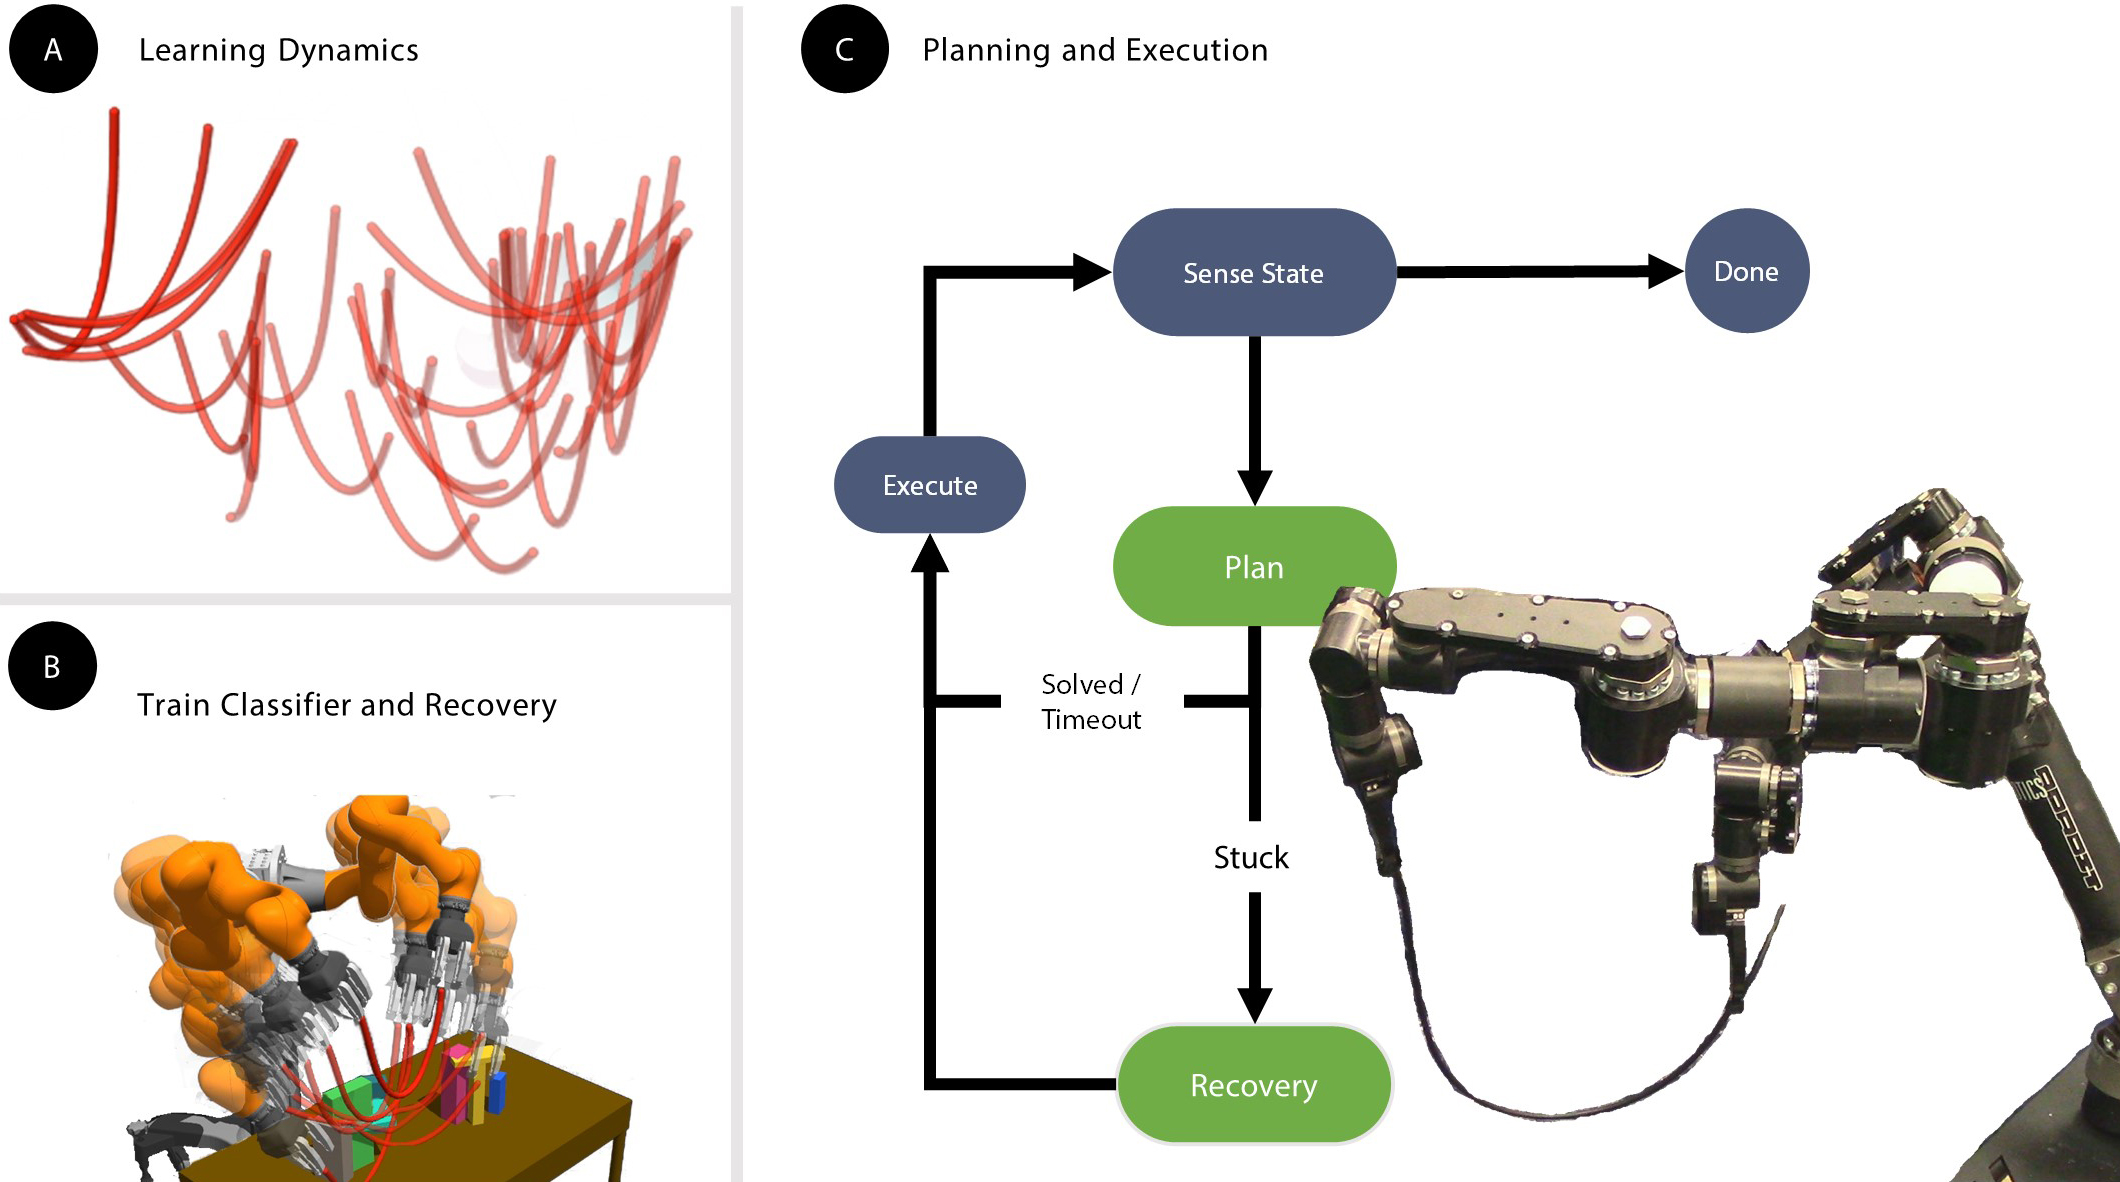
\includegraphics[width=0.8\linewidth]{Chap2/images/figure1}
    \caption{Overview of the proposed method. Two data collection phases (A,B) are used to collect training data for learning dynamics, a classifier for where these dynamics are accurate, and a recovery model what for actions to take when no accurate dynamics predictions can be made. These learned components are used in an iterative process of planning, replanning, and recovery (C). We apply this method to a number of deformable objects tasks, including a dual arm robot manipulating an automotive hose.}
    \label{Scirob:fig:figure1}
\end{figure}
\section{Problem Statement} \label{SciRob:sec:problem}

Here we present the formal problem addressed by our method. Let the state space of the system be $\statespace$ and the action space be $\actionSpace$. The true dynamics are $\worlddynamicsdef$ produces the next state $\nextstate$ given the environment $\env$, state $\currentstate$, and action $\currentaction$. We consider the feasible discrete-time motion planning problem, which informally means finding a sequence of actions that take the system from a start configuration $\state^0$ to a goal region $\goal \subset \statespace$. In general, $\worlddynamics$ may not be known in closed-form, or it may be expensive to evaluate within a planner. Thus, we cannot solve this problem by planning with the true dynamics $\worlddynamics$.

Instead, we consider the challenge of planning with an incomplete model of the dynamics $\ourdynamics$. Since these dynamics will sometimes be inaccurate, we introduce the model-error requirement (MER) to reason about where they can be trusted. The MER is a constraint in the planning problem, to ensure that our plan only contains predictions from our dynamics $\ourdynamics$ that are $\modelerrorthreshold$-close to the true dynamics $\worlddynamics$. The model-error is defined for a given state-action $(\currentstate,\currentaction)$ using a distance function in state space $\distfname$, and is shown in Equation \eqref{Scirob:eq:modelerror}.

\begin{equation}
\modelerrordef
\label{Scirob:eq:modelerror}
\end{equation}

Using this, we define the MER itself as $\MER$. Thus, the planning problem is

\begin{equation}
  \begin{array}{ccll}
    \find & \horizon,\action^0,\dots,\lastaction & \\
    \subjectto & \nextstatepred = \ourdynamicsfunc & t \in [0,\horizon) \\
    & \modelerrorconstraint & t \in [0,\horizon) \\
    & \laststatepred \in \goal & \\
  \end{array}
  \label{Scirob:eq:planning_problem}
\end{equation}

\subsection{Classifier}

We cannot evaluate the MER directly during planning because it requires the true future state $\nextstate$.
In planning, we only know the environment, actions, and predicted states $(\env,\currentstatepred,\currentaction,\nextstatepred)$. Consequently, we need to evaluate the MER using only the information known in planning. This can be posed as the following binary classification problem:
\begin{equation}
  \begin{array}{rl}
    \classifierInputs & \env,\currentstatepred,\currentaction,\nextstatepred \\
    \classifierLabel & \MER \\
  \end{array}
  \label{Scirob:eq:strict_mer_classification_problem}
\end{equation}

Let the classifier which solves this problem be $\classifierdefNoVar$. For training this classifier, \classifierLabel can be computed using the actual $\nextstate$ recorded during data collection (Section ``\nameref{Scirob:sec:phase_two_collection}''). A diagram illustrating the inputs to the classifier and its labels is shown in Figure \ref{Scirob:fig:figure3}. Finally, given dynamics $\ourdynamics$ and classifier $\classifier$, we can approximately solve Problem \eqref{Scirob:eq:planning_problem} using motion planning (see Section ``\nameref{Scirob:sec:planning}'').

We note that the MER is conservative in the sense that we only need the final predicted $\laststatepred$ and actual state $\laststate$ to be close. Unfortunately, reasoning about only the final state in the MER would be a constraint on the entire trajectory. Such a constraint is neither tractable to learn nor amenable to planning in our scenarios. Thus, we enforce the MER for every action taken by the planner.

\begin{figure}
    \centering
    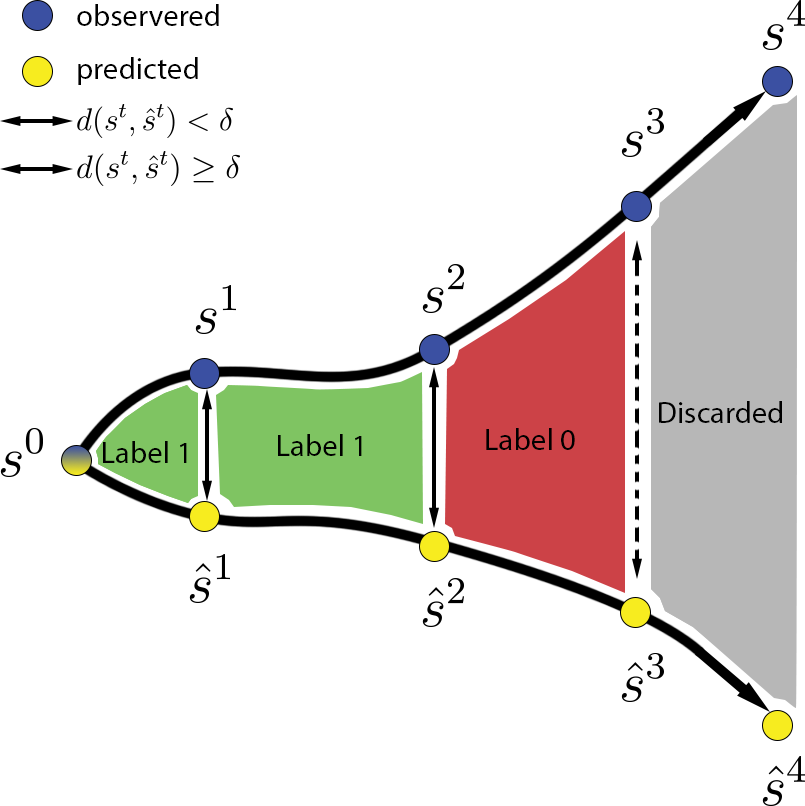
\includegraphics[width=0.5\linewidth]{Chap2/images/figure3-v2}
    \caption{Converting a trajectory into examples for training the classifier. Each large box represents a transition. In the first transition, the final states $\state^1$ and $\statepred^1$ are close, so the transition is labeled 1 (accurate). For the third transition, the initial states $\state^2$ and $\statepred^2$ are close, but the final states $\state^3$ and $\statepred^3$ are far, so this transition is labeled 0 (inaccurate). In the final transition, the initial states are far, so this transition is discarded.}
    \label{Scirob:fig:figure3}
\end{figure}

\subsection{Recovery}

With this definition of the MER and the classifier, we also formally define what it means to be stuck, i.e. in need of recovery. This can be written as a function $\recoverydef$ which determines whether a given state, environment pair can be escaped while enforcing the MER: 
\begin{equation}
    \recoveryfuncfull
    = \begin{cases}
    0 & \exists\,\action \in \actionSpace\ \text{for which}\ \MER \\
    1 & \text{otherwise}
    \end{cases} \\
    \label{Scirob:eq:recovery}
\end{equation}

Again, we cannot compute $\recoveryfuncfull$ directly online, as it requires knowing the actual effect of executing actions. Instead, we will use an approximation to this function. Once we know if a state is in need of recovery, we can either launch the planner (if not) or perform recovery actions (if so).

\subsection{State Definition}

In this chapter, we focus on rope manipulation tasks with $\NGrippers=1$ or $\NGrippers=2$ grippers; the state of each gripper is a point in $\reals^3$. We assume that the robot end effectors are rigidly attached to the object. The configuration of the rope is a set of $\NLinks$ points in $\reals^{3\NLinks}$. The state $s$ is then a vector of the positions of the gripper(s) and the points along the rope. The dimension of the state space is thus $\Ndim = 3 (\NGrippers + \NLinks )$.

\section{Methods} \label{SciRob:sec:methods}

\begin{figure}
    \centering
    \includegraphics[width=0.8\linewidth]{Chap2/images/figure2}
    \caption{Pictures of our simulation and real robot scenarios. (A) Simulated Rope Dragging. (B) Simulated Tabletop Rope Manipulation. (C) Retrieving a Charging Cable. (D) Removing Lifting Straps. (E) Moving a Hose. (F) Preparing to Install a Hose. Annotations show examples of goals for various tasks our method can complete.}
    \label{Scirob:fig:figure2}
\end{figure}


\subsection{Data Collection for Learning the Dynamics}

\label{Scirob:sec:phase_one_collection}
Our first phase of data collection is used for training our model of the unconstrained dynamics. This involves sampling random actions and recording the observed states to form trajectories $[\state^0,\action^0,\state^1,\dots,\lasttrainaction,\lasttrainstate]$. In all our experiments, we use $\trainhorizon=10$. We sample actions randomly, choosing target positions which are within \SI{0.1}{\meter} of the current gripper position(s). Put another way, we sample actions which are changes in position in a ball around the current position. We repeat the previously sampled change in position with 80\% probability, which creates larger, more consistent motions and gives better coverage of our environments. During this phase, we do not reset the rope's position between trajectories.

In this phase, we also want to avoid activating physical constraints during data collection. This is done by removing obstacles, and by restricting the actions taken during data collection. For rope dragging, this only means removing any obstacles. For dual arm rope manipulation, this means removing obstacles, removing the arms entirely, and preventing the rope from overstretching by limiting the distance between the grippers. Although removing the arms would not be possible in the real world, it seems possible to design a conservative set of actions which would similarly ensure that the rope does not interact with the arms, or the arms with each other. At a high level, the purpose of this is to simplify the dynamics by avoiding activating any physical constraints during this phase.

For rope dragging, we collected 6,144 trajectories containing 10 steps, of which 1,536 are reserved for validation and testing. For dual arm rope manipulation, we collected 2,048 trajectories containing 10 steps, of which 512 are reserved for validation and testing.
\subsection{Learning the Unconstrained Dynamics}
\label{Scirob:sec:learning_dynamics}

Once we have collected our dataset of trajectories, we train our dynamics network. This network is a two layer fully connected neural network which takes in a state $\currentstate$ and action $\currentaction$ and predicts a change in state $\Delta \nextstatepred$. A diagram showing this architecture is shown in Figure \ref{Scirob:fig:figure4} and discussed in more detail in Section ``\nameref{Scirob:sec:architectures}''. This model can be used to make multistep predictions by feeding the predicted state back into the model. The loss is the combined prediction error for all time steps in the trajectory, and is shown in Equation \eqref{Scirob:eq:dyn_loss}.

\begin{equation}
	\begin{split}
	MSE(\state^0, \action^0, \dots, \lasttrainaction) &= \frac{1}{\trainhorizon} \sum_{t=1}^{\trainhorizon-1} \left\| \currentstatepred - \currentstate \right\|^2 \\
	\statepred^0 &= \state^0 \\
	\nextstatepred &= \ourdynamics(\env, \currentstatepred, \currentaction)
	\end{split}
	\label{Scirob:eq:dyn_loss}
\end{equation}

\subsubsection{Incorporating Uncertainty in the Learned Dynamics}
\label{Scirob:sec:uncertainty}

Prior work has shown that it can be beneficial to consider the uncertainty in the learned dynamics \cite{Schneider1996,Bechtle2019,Chua2018}, even without considering constraints not seen in training. For instance, if the training data does not cover the state-action space well, then having a measure of uncertainty in the dynamics predictions makes it possible to detect out of distribution predictions. This is a measure of \textit{epistemic uncertainty}---uncertainty due to lack of data (as opposed to inherent randomness) \cite{Hullermeier2021,Hora1996}.

As is done in prior work \cite{Gal2016,Chua2018,Lakshminarayanan2017}, we use an ensemble of neural networks trained on the same phase one data starting with different random seeds. When a point prediction is needed, like in planning or in constructing the classifier and recovery datasets, we take the mean of the ensemble prediction. When a measure of uncertainty is needed, we compute the sum of the standard deviations along each dimension of state across all the models in the ensemble. For simplicity we will denote this as $\variance$. We use this measure of uncertainty as an input to the classifier. The intuition behind this method is that the trained networks' predictions will be similar near the training data, but will diverge far away from training data. This makes it possible for the classifier to reject or accept transitions based on the uncertainty of the learned dynamics. Although we did not find that this provided a significant improvement for our tasks, we include it nonetheless as it may be beneficial in scenarios where the unconstrained model is trained on a dataset with poor coverage of the state space.

\subsection{Phase Two Data Collection}
\label{Scirob:sec:phase_two_collection}

Once the unconstrained dynamics have been learned, we next learn where this model is accurate, and what actions to take when it is not. For this, we perform a second phase of data collection. In this phase, we collect data in the kinds of environments where we intend to perform tasks. We perform the same type of random data collection process as in the first phase, but now physical constraints are included, allowing us to gather examples of where our unconstrained dynamics are accurate and where they are not. Using the data collected in this phase, we can construct datasets to train our classifier as well as our recovery actions model. A related approach was used in \cite{Guzzi2020} for learning to estimate the reachability of a quadruped robot. Our prior work has also demonstrated that this type of data can also be collected by planning and executing those plans, rather than by taking random actions \cite{McConachie2020}. However, both of the above methods used analytical/simulation models for predicting the dynamics. Furthermore, our approach is in contrast to many methods in robust control and safe reinforcement learning, which are built on the idea that predictions made outside the training distribution are unreliable \cite{Zhou1998,Gal2016}. Those methods do not require a second data collection phase, but as a consequence would be overly conservative as the presence of any obstacle near the rope would be considered out-of-distribution.

In order to get diverse data we frequently randomize the locations of obstacles in the environment. For dual arm rope manipulation, this requires releasing the rope and moving the arms out of the way before randomizing obstacles, so that we can arrange the obstacles without permanently entangling the rope or arms.

For rope dragging, we collected 2,048 trajectories of length 50 in phase two, of which 512 were reserved for validation and testing. For dual arm rope manipulation, we collected 5,996 trajectories of length 20, of which 1,516 were reserved for validation and testing.

In total, the combined phase one and two datasets for dragging has 163,840 transitions, and the combined phase one two datasets for dual arm rope manipulation has 140,400 transitions. In comparison, \cite{Propnet} uses 500,000 transitions in order to accurately learn the contact dynamics of a rope amongst disc-shaped obstacles in 2D.

\subsection{Learning the Classifier}
\label{Scirob:sec:learning_classifier}

Given the data collected in phase two, we now describe how to construct training examples for the classifier. For this we need both the predictions of the unconstrained dynamics as well the labels of whether the model-error requirement is satisfied. To compute the predictions, we take the starting state for each trajectory in the dataset and roll out the unconstrained dynamics prediction for the rest of the trajectory. This produces a tuple of $(\currentstate, \currentstatepred, \currentaction, \nextstate, \nextstatepred)$ for each time step in each trajectory. As stated in Problem $\eqref{Scirob:eq:planning_problem}$ the label should be 1 if $\modelerrorconstraint$ and 0 otherwise. To compute $\modelerror$, we require a distance function $\distfname$ between the predicted state $\nextstatepred$ and the actual state $\nextstate$. We selected the threshold $\modelerrorthreshold$ by computing the 90th percentile of prediction error for the unconstrained dynamics on the unconstrained dynamics validation set. A sensitivity analysis of the threshold is given in Supplementary Materials. For rope dragging, $\modelerrorthreshold=$\SI{0.065}{\meter} and for dual arm rope manipulation $\modelerrorthreshold=$\SI{0.025}{\meter}. Additionally, we discard all the transitions after the first transition labeled 0, since it is unclear whether the dynamics would have been accurate had it not diverged previously. A diagram illustrating how a trajectory is converted into examples for the classifier is shown in Figure \ref{Scirob:fig:3DClassifierInput}.

\begin{figure}
    \centering
    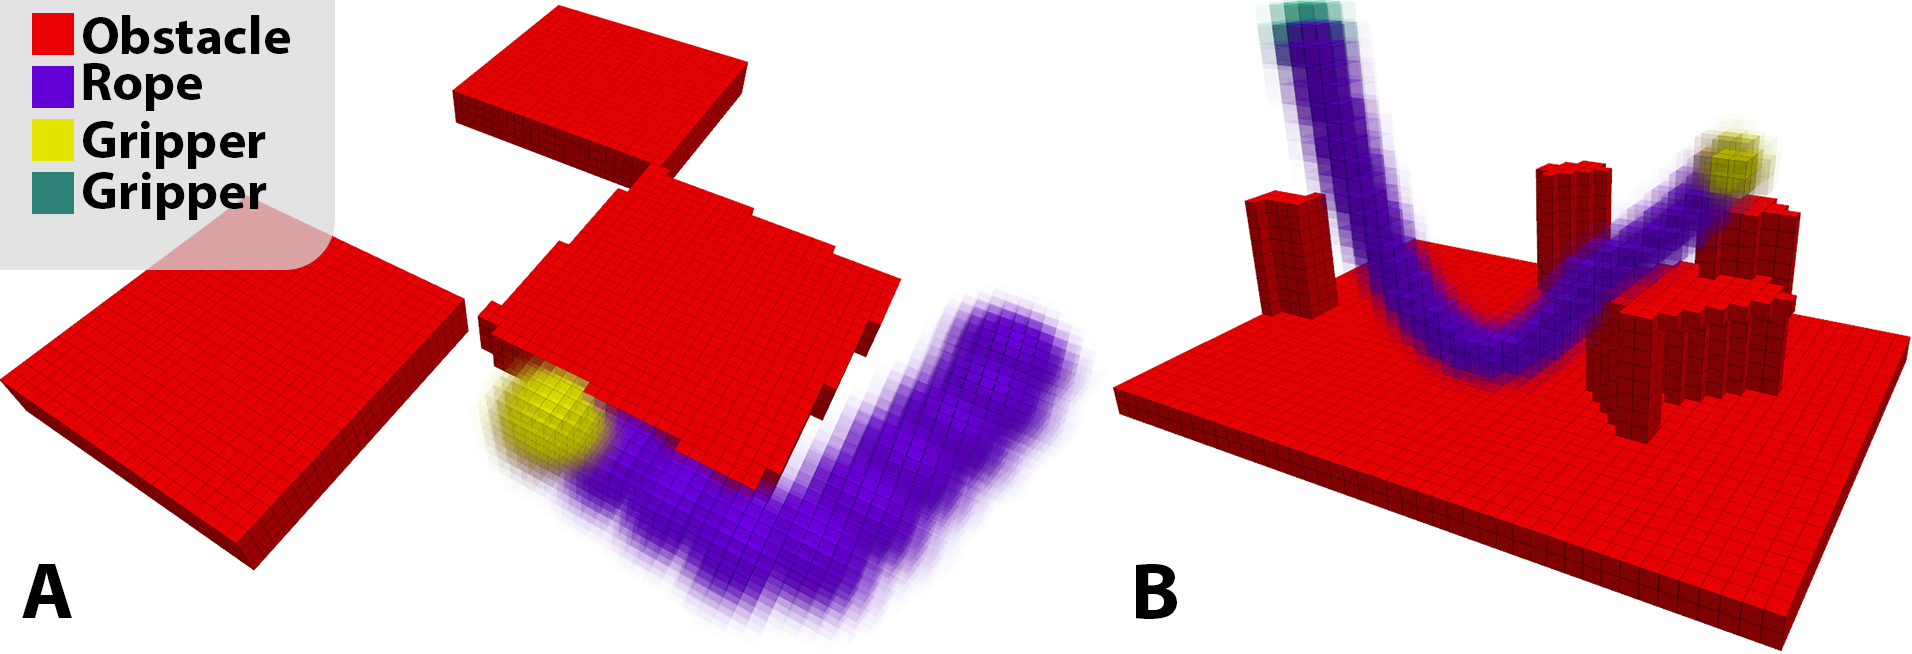
\includegraphics[width=0.6\linewidth]{Chap2/images/figure5}
    \caption{Representing the state and environment in 3D voxel grids. (A) An example for rope dragging. (B) An example dual arm rope manipulation. Different colors are used to represent different channels in the voxel grid, and alpha is used to indicate the voxel value, with 0 being fully transparent and 1 being fully opaque.}
    \label{Scirob:fig:3DClassifierInput}
\end{figure}

The classifier network $\classifierdef$ takes as input the environment $\env$ and the transition $\currentstatepred,\currentaction,\nextstatepred$. Since we use an ensemble of dynamics models, these states are the mean predictions of the ensemble. We also include the variance $\variance$ of the ensemble predictions as input to the classifier. The classifier outputs a number between 0 (inaccurate) and 1 (accurate). The network architecture is shown in Figure \ref{Scirob:fig:figure4}. Since this is a binary classification problem, we use binary cross-entropy loss to train it. Furthermore, since physical constraints are spatial in nature, we convert the environment and states into multi-channel 3D voxel grids and use Convolutional Neural Networks (CNN) (details in Section ``\nameref{Scirob:sec:architectures}'').

We also note that depending on the environments and specific parameters for how actions are sampled, the resulting dataset of transitions may be imbalanced. In our experiments, our classifier datasets contained more positive than negative examples, ranging between 65\% and 95\% positive. To mitigate bias in our classifier, we balance each minibatch by oversampling examples from the underrepresented class.

\subsection{Planning With a Learned Model and Classifier}
\label{Scirob:sec:planning}

Once we have learned our unconstrained dynamics and classifier, these models are used for planning. Although they could be applied to a number of different planning methods, including the cross entropy method (CEM) \cite{Kobilarov2011}, probabilistic roadmaps (PRM) \cite{Kavraki1996}, or trajectory optimization \cite{Ratliff2006}, we chose to use them in a kinodynamic RRT \cite{LaValle2001}, as implemented in the Open Motion Planning Library (OMPL) \cite{ompl}. Kinodynamic RRT is a sampling-based tree-search algorithm, and is well suited for our tasks as they contain local minima and narrow passages. Graph-based methods like PRMs could be used instead if we expect to plan repeatedly in the same environment, and trajectory optimization could be used if there are criteria such as path length which should be minimized.

In our Kinodynamic RRT, we sample a single random action $\currentaction$ and attempt to extend using that action. Whenever we attempt to extend from state $\currentstatepred$ with action $\currentaction$ to the state $\nextstatepred$, we first check the transition $(\currentstatepred,\currentaction,\nextstatepred)$ by feeding it through the classifier. The extension is added to the tree only if the classifier output is greater than $\paccept$. We chose this type of planner for its simplicity, and many algorithmic and implementation optimizations could be made to decrease planning times.

\subsection{Evaluating Stuck States and Learning Recovery}
\label{Scirob:sec:learning_recovery}

The formal definition of being stuck (Equation \eqref{Scirob:eq:recovery}) evaluates every possible action from a given state. In practice, checking whether a state is stuck consists of sampling $\NRecoverySamples$ actions and checking whether any of them are accepted by the classifier. Since the classifier is trained to approximate the MER, this is a quick and effective method for determining whether recovery is needed. Additionally, this procedure is done naturally by the RRT at the start of planning, which means that checking for recovery can be easily integrated into planning without any redundant calls to sampling, dynamics, or classification.

Given the unconstrained dynamics and the classifier, we can also use the data collected in phase two to learn recovery actions. As defined in our problem statement, recovery actions are needed when the robot is in a state where the classifier rejects all proposed actions. In this case, we would like the robot to take \textit{recovery actions} which bring it back to regions of state space where the unconstrained dynamics are accurate.

For this, we propose training a neural network to evaluate the probability that an action is recovering. This network takes in a state, action, and the environment $\recovInputs$ and outputs the probability $\recovProb$ that the action is recovering. Specifically, when we detect recovery is needed, we sample $\NRecoverySamples$ actions randomly and use this learned recovery model to assign each action a probability of recovering. The highest probability action is then selected and executed; this sampling, recovery probability evaluation, and execution process repeats until the system is no longer stuck. This approach requires training a model which estimates the probability that an action is recovering. To construct a dataset of recovering actions and labels of the recovery probability, we use a similar approach to the one used to construct the classifier dataset.

This process considers each observed transition $\currentstate,\currentaction,\nextstate$ and environment $\env$ in the dataset and first determines whether recovery is needed at $\currentstate$. We sample $\NRecoverySamples$ random actions from that state, predict according to the unconstrained dynamics, and feed this into the classifier. If all $\NRecoverySamples$ sampled transitions are rejected, then the state $\currentstate$ needs recovery. Next we perform the same test starting at the next state $\nextstate$. Here we record the proportion of the sampled actions which were accepted, and this is used as the label for probability of recovery $\recovProb$. For example, if at $\currentstate$ none of the random samples were accepted, but from $\nextstate$ all $\NRecoverySamples$ were accepted, then this is an excellent example of recovery, and we would like our recovery model to predict that taking action $\currentaction$ from $\currentstate$ in environment $\env$ is likely to lead to recovery. On the other hand, if when checking $\nextstate$ we find that still no actions are accepted by the classifier, then this is a poor example of recovery. We use all transitions for which recovery is needed (i.e. $\recoveryfuncfull = 1$ as the dataset for training our recovery model, and train the network using binary-cross entropy to predict the recovery probability. For our experiments, we set $\NRecoverySamples$ to 32. More details about the neural network and its structure can be found in Section ``\nameref{Scirob:sec:architectures}''.

Approaches to recovery like those from the safe exploration community \cite{Koller2018,Berkenkamp2017,Fisac2019safety} are focused on staying within a region of the state space from which the agent can guarantee safety during the learning process, or the existence of a sequence of control actions which will move the system into a predefined safe set. In contrast, our method is targeting the case where the model is already too unreliable for use at the given state and any predictions made cannot be trusted.

\subsection{Network architectures}
\label{Scirob:sec:architectures}

\begin{figure}
    \centering
    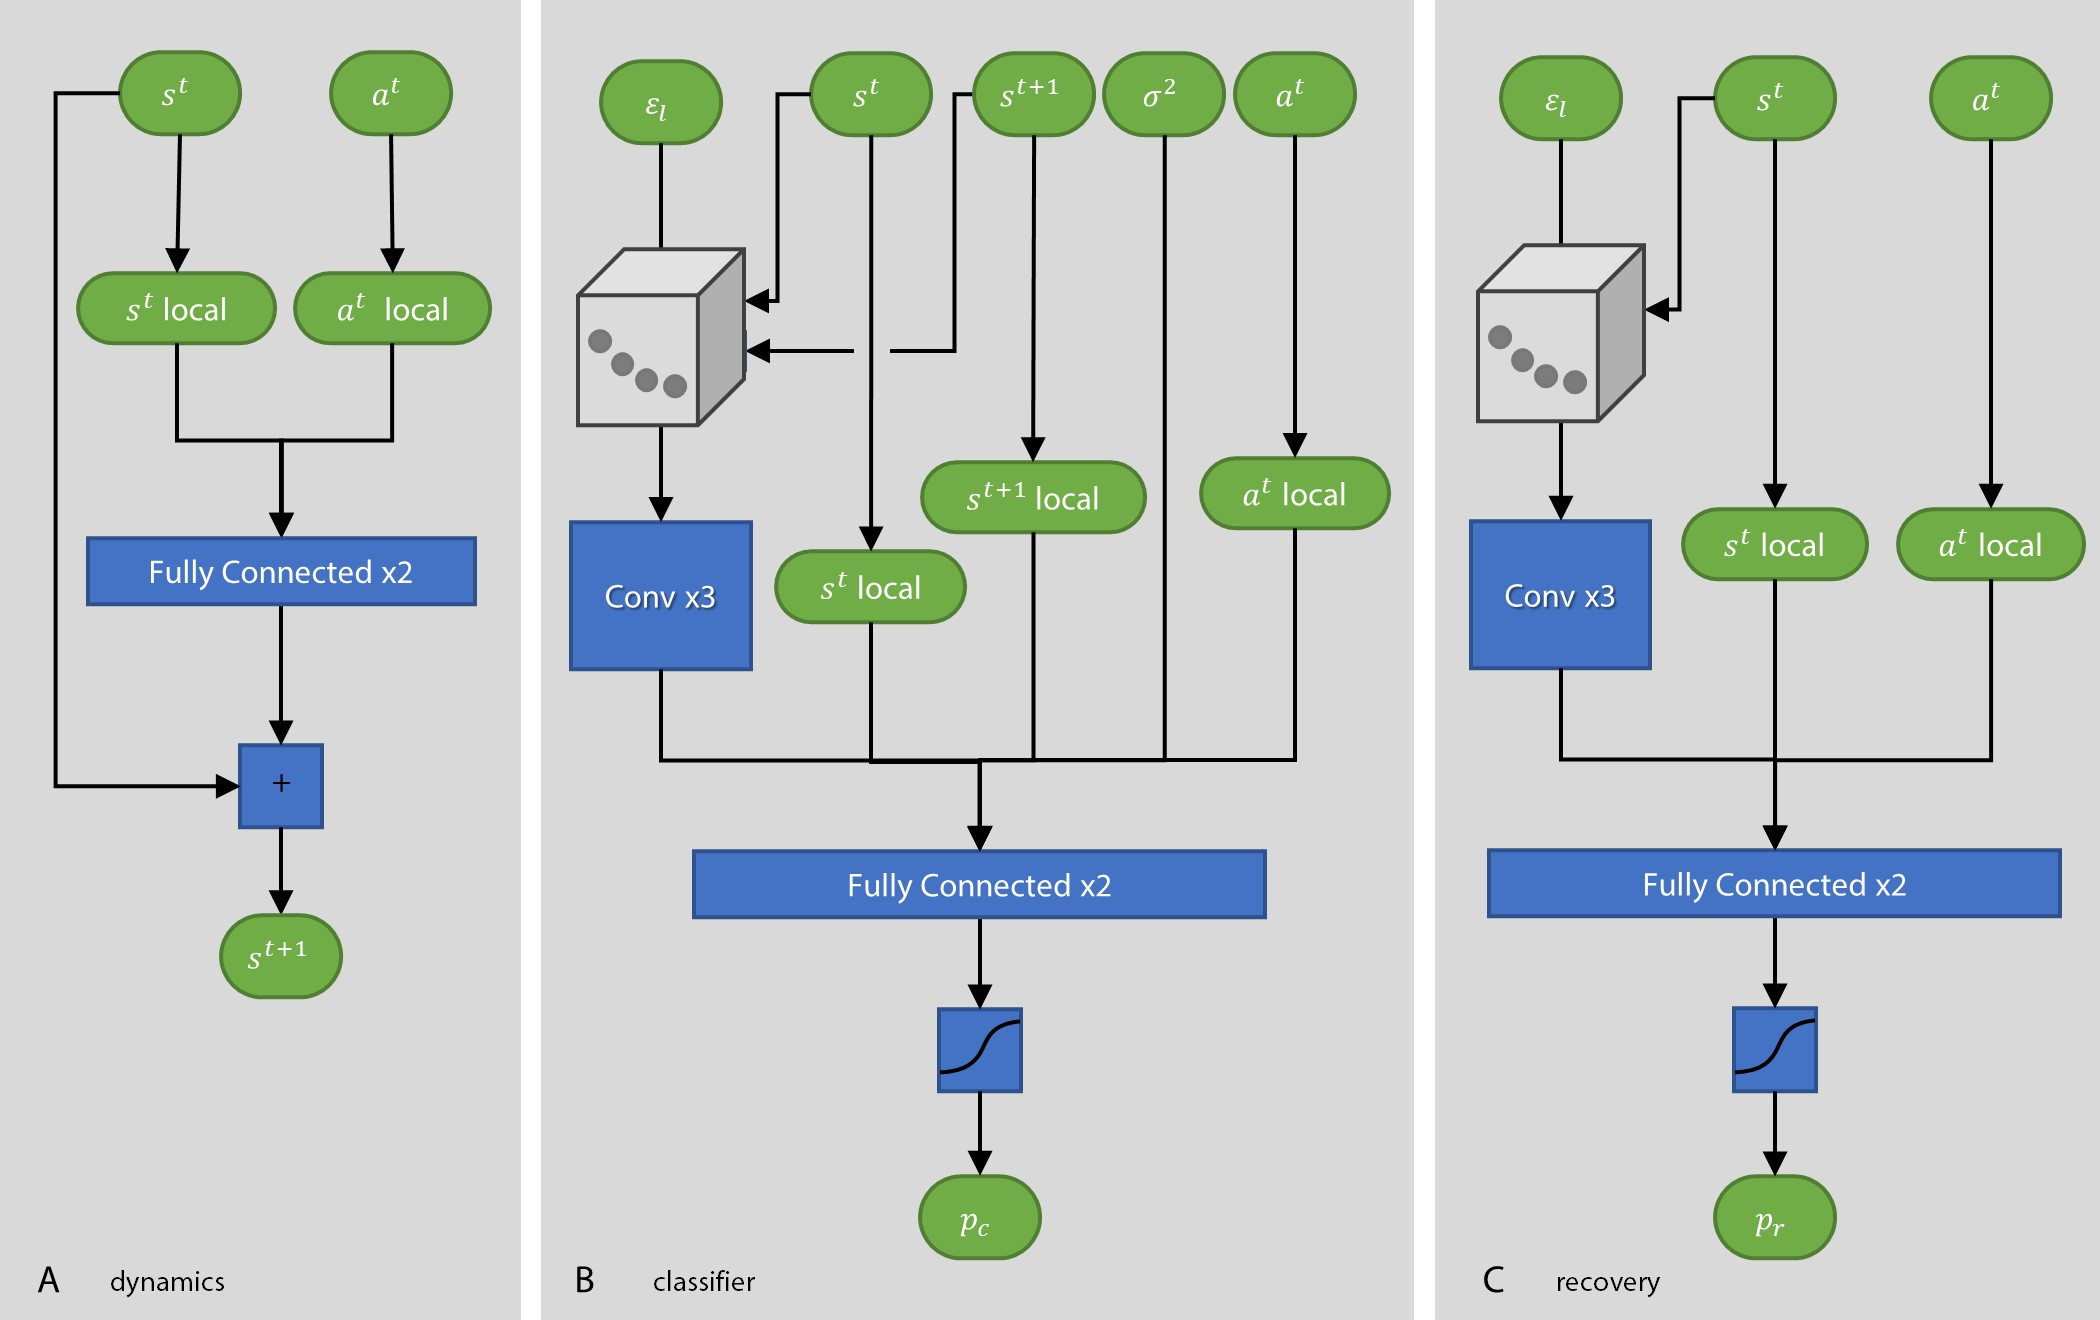
\includegraphics[width=0.7\linewidth]{Chap2/images/figure4}
    \caption{Network architectures. (A) dynamics, (B) classifier, and (C) recovery. \textit{local} refers to the translations used to make the states and actions invariant to the position in the world frame, and is described in Sections ``\nameref{Scirob:sec:learning_dynamics}'', ``\nameref{Scirob:sec:learning_classifier}'', and ``\nameref{Scirob:sec:architectures}''. Green capsules shapes indicate vectors, and blue boxes indicate functions. The gray 3D box represents the 3D voxel grid representation of state (Section ``\nameref{Scirob:sec:voxels}'').}
    \label{Scirob:fig:figure4}
\end{figure}

Our method uses three neural networks, one for the dynamics model, one for the classifier, and one for recovery. Architectures are shown in Figure \ref{Scirob:fig:figure4}.

\subsubsection{Dynamics Model Architecture}

The dynamics network is a two layer fully connected network with 1,024 hidden units in each layer and ReLU activation. This model takes in the state of the rope and grippers concatenated with the actions and outputs the change in state, which is then added to the input state to produce the final predicted state. Furthermore, because we assume that the unconstrained dynamics are invariant to the global position in space, we first translate the state and actions into a local frame before feeding them into the dynamics network. For rope dragging, states and actions are relative to the position of the gripper, and for dual arm manipulation they are relative to the average of all the points of the rope. 

\subsubsection{Classifier Architecture}

The classifier network takes in the environment $\env$ and a transition $\transitionpred$ and outputs the probability of the MER being satisfied. Since we experimented with performing classification on multiple transitions we use a Long Short Term Memory network (LSTM) with a CNN encoder, although in this work we only consider a single transition as input. As shown in Figure \ref{Scirob:fig:figure4}, a single time step is passed through a CNN encoder that maps a single state $\currentstatepred$ and action $\currentaction$ into a latent vector. The state and environment are first represented in a 3D voxel grid and passed through three convolutional layers. The output is flattened and concatenated with the vector representations of the state and action. The LSTM outputs a scalar prediction of the probability of the MER being satisfied for each time step. Since we use a single transition, this means there are two outputs, one for time $t$ and one for $t+1$. The output for time $t$ is ignored, because it is not a function of $\nextstatepred$. Instead, we use the output for time $t+1$ as the probability for the entire transition $\transitionpred$.

\label{Scirob:sec:voxels}
In order to represent the environment and states in a voxel grid of a fixed size, we take a crop of the full environment occupancy grid centered around the local origin (as defined above for dynamics). As with the local representation of states and actions, this assumes invariance to the absolute position. Additionally, using a fixed size local environment has the benefit of allowing the size of the full environment to change from task to task without any retraining. In order to make it easier for the classifier to reason over the 3D input, we also include a 3D representation of the input states. For each component of the state (grippers, rope) we construct a 3D voxel grid of the same size and location as the local environment and each voxel's value is proportional to the inverse-log of its distance to the nearest point in that component of the state. This results in a smoothed version of simply drawing the points into the voxel grid, and examples are shown in Figure \ref{Scirob:fig:3DClassifierInput}. We stack these representations along with the local environment to get a multi-channel voxel grid.

The vector representations of state and action are the same as is described for the dynamics, however we use both the original state vector (not translated) and the local state vector (translated). This is because the classifier should be able to learn reachability and kinematic constraints, e.g. in our dual-arm manipulation scenario. 

\subsubsection{Recovery Architecture}

Finally, the recovery network has the same encoder structure as the classifier, and we use the learned parameters, without fine-tuning, of convolution layers from the classifier in the recovery network. This network takes in a proposed transition, this time consisting of the 3D local environment, a single state, and a proposed action, and outputs the probability of recovery. Unlike the classifier, we do not pass in the predicted result of the proposed action, since recovery is only used when accurate predictions cannot be made. After encoding, two fully connected layer with ReLU activation followed by a layer with sigmoid activation are used to map down to the output probability.

\subsubsection{Full Dynamics Architecture}

Our full dynamics baseline uses a different network. We use the network proposed in \cite{NagabandiImageConditiondDynamics2018}, but extend to 3D convolution. The state representations used are the same as in our unconstrained dynamics network. Graph neural network architectures for predicting physics in 3D may provide more accurate predictions \cite{Propnet,Mrowca2018}, however these networks assume a graphical model of the world is known, whereas our dynamics learning method does not.

\subsection{Simulation Environments}
\label{Scirob:sec:sim_envs}

We use the Gazebo simulator with ODE physics \cite{Gazebo,ODE} for our quantitative experiments. We emphasize that our method does not have access to the simulator's model of the rope or the simulation parameters. For our rope dragging experiment, the rope is modeled with 10 rigid links, and the state consists of the positions of the links and the position of the gripper $\state=[x_g,y_g,z_g,x_1,y_1,z_1,\dots,x_{10},y_{10},z_{10}]$, which has 33 dimensions.
We considered including gripper orientation, however this would make the dynamics dependent on gripper geometry and friction properties (because the rope could wind around the gripper) without necessarily enabling significant new capabilities, so we chose not to include orientation. The gripper is attached to one end of the rope, and the point at the other end of the rope (which we will call the tail) is the point which we wish to place at a goal position. Task error is measured is the Euclidean distance in 3D between the tail and the goal point. The actions are target gripper positions $\action = [x,y,z]$, and a local controller is used to attempt to reach these goals. When commanded into an obstacle, the gripper will stop or potentially slide as it applies force into the obstacle. An action completes when the commanded position is reached or a timeout of 1 second occurs. The nominal joint velocity of the controller is tuned to reduce jerk and keep the simulation quasi-static.

For the dual arm rope manipulation experiments, the rope is modeled with 25 rigid links, and the state consists of the positions of the links and the positions of the two grippers $\state=[x_{g1},y_{g1},z_{g1},x_{g2},y_{g2},z_{g2},x_1,y_1,z_1,\dots,x_{25},y_{25},z_{25}]$, which has 81 dimensions.
The grippers attach to opposite ends of the rope. The actions are target positions for each gripper $\action = [x_1,y_1,z_1,x_2,y_2,z_2]$. A Jacobian-based inverse kinematics controller is used to track the target position for each gripper. This controller stops when the target position is reached or just before any collisions between the arms or between the arms and obstacles.
\section{Discussion} \label{SciRob:sec:discussion}

\subsection{On the Specialization to Deformable Objects}
Planning with inaccurate models has many potential applications, so it would be interesting to explore a broader range of tasks in future work. However, deformable object manipulation is particularly well-suited for our framework. Specifically because  1) Compliance allows us to make mistakes, stop, and replan; 2) Dynamics are more complex in some regions than in others; and 3) Much of the state space and dynamics are irrelevant for doing useful tasks. We discuss each of these points below:

First, our method relies on taking actions for which we have no accurate model, which means we must be able to take actions safely, despite their outcome being uncertain. The compliance afforded by deformable objects allows us to safely collect data, and thus to learn where our model is wrong.

Second, our method assumes that there is some subset of the dynamics which we can learn accurately, and which is sufficiently useful. Such an assumption is particularly well-suited to deformable object manipulation, where the full dynamics are much more difficult to learn than the unconstrained dynamics, yet interesting and practical tasks can still be done without learning these dynamics.

Third, deformable objects have high-dimensional state-action spaces. However, only a small region of state-action space is either reachable or useful for practical tasks (i.e. we need not consider the many different crumpled or knotted states). Because of this, it is often acceptable to avoid large portions of this space. Our method takes advantage of this in many ways, including 1) only learning the dynamics for the subset of state-action space covered in phase 1 data collection, and 2) only learning the classifier for the relatively small subset of state-action space covered in phase 2 data collection.

\subsection{Limitations} In this work we present significant progress on planning with unreliable models and addressing their inaccuracies, however many open questions remain. In this work we do not address challenges in state estimation and tracking, control and precise manipulation, or in describing and defining complex tasks.

There are also many avenues in which our proposed methods might be improved or extended. For instance, we define which simplified dynamics should be learned by defining the phase one setting and data collection procedures. This assumes that we know which dynamics will be tractable to learn, but still useful for planning in more constrained scenarios. In future work, it would be interesting to explore how to make this decision automatically, e.g. we can search over various simplifications of the dynamics based on the performance of learned models. Finally, we plan to extend these methods to incorporate real world data based on potentially unreliable perception and tracking.

Although we show that our method can be used for several interesting tasks, we are limiting the tasks our method can do by choosing to learn only the unconstrained dynamics. Our method assumes that the goal is reachable while remaining in the part of state-action space where the unconstrained dynamics are accurate. While this is a reasonable assumption, it would be interesting to incorporate our method into a framework which uses it to get as close as possible to a given goal and then switching to a feedback-based local method (e.g. \cite{LinearAlarcon2013,Jia2018,Wu2020}) to finalize the task (as is done in \cite{McConachie2020}).

In terms of recovery, we note that although our learned recovery actions dramatically improved our performance for the dual arm manipulation task, the learned recovery policy still fails in some cases. The learned recovery policy tends to raise the grippers, as this is an effective strategy in the training data. However, while this will work well when the rope is draped on the table or obstacles, it leads to being caught on a protrusion if the rope starts below it. A better policy would likely be learned by collecting phase two data in environments where getting caught and escaping is more likely. 

In this work, we treat the simulator as a black-box proxy for the real world. However, these simulations can differ from real world physics, and so at best they provide a starting point from which sim2real methods can be used to transfer either a learned dynamics model \cite{Fu2016,Clavera2018} or a learned policy \cite{Bousmalis2018,Peng2018} to the real world. For instance, it would be useful to adapt online to different stiffnesses of lengths of rope without re-collecting large datasets. Sim2real has been demonstrated for a number of other robots and tasks \cite{Lee2020,OpenAI2019}, and incorporating these techniques into our proposed methods is an interesting direction for future work.
\subsection{Learning Performance}
In addition to reporting the performance of our complete method on various tasks, here we also report the training and validation accuracies of our learned models. Further details on the training of these models can be found in Sections ``\nameref{Scirob:sec:learning_dynamics}'', ``\nameref{Scirob:sec:learning_classifier}'', and ``\nameref{Scirob:sec:learning_recovery}''.

For dynamics learning, we report learning error as the Euclidean distance between every predicted and true point on the rope, and average over all the points, time steps, and examples in the dataset. For rope dragging, our unconstrained dynamics model has an error of \SI{0.0081}{\meter} in training and \SI{0.0097}{\meter} in testing. These numbers are small in comparison to the length of the rope (\SI{0.5}{\meter}) and the size of the environment (2x2m). For a visual demonstration of this level of error,r please see our video. FD achieves an error of \SI{0.0090}{\meter} in training and \SI{0.0117}{\meter} in testing. For dual arm rope manipulation, our unconstrained dynamics model has an error of \SI{0.0025}{\meter} in training in \SI{0.0030}{\meter} in testing. Here the rope has a length of \SI{0.8}{\meter}, indicating that we are able to learn the unconstrained dynamics very accurately. The full dynamics baseline achieves an error of \SI{0.0194}{\meter} in training and \SI{0.0218}{\meter} in testing. Learning accurate dynamics over long horizons is critical for planning, and by learning only the unconstrained dynamics, our method is able to do so with higher accuracy than the full dynamics baseline.

We report learning metrics on the phase two dataset (see Section ``\nameref{Scirob:sec:learning_classifier}'' for details). For rope dragging, the classifier achieved an accuracy of $0.890$, precision of $0.959$ and recall of $0.822$ on the training set. On the testing set, it has an accuracy of $0.835$, precision of $0.888$, and recall of $0.789$. For dual arm rope manipulation, the classifier achieved an accuracy of $0.904$, precision of $0.914$ and recall of $0.927$ on the training set. On the testing set, it has an accuracy of $0.890$, precision of $0.895$, and recall of $0.927$. Throughout our experimentation we observed that, as prior work has noted \cite{McConachie2020}, the accuracy of this classifier is a poor indicator of its usefulness in planning.

For recovery, we use the binary cross entropy loss to measure learning performance. For rope dragging, the training loss (unitless) is $0.021$ and the testing loss is $0.023$. For rope dragging, the training loss is $0.139$ and the testing loss is $0.146$. 

\subsection{Physical Robot Demonstrations}
\label{Scirob:sec:physical_robot_details}
To demonstrate the practicality of our method, we designed real-world mockups of domestic and automotive tasks. For dual arm manipulation, we demonstrate three tasks done under the hood of a car, where the robot manipulates hoses and straps. For rope dragging we show an example where the robot retrieves a phone charging cable by sliding it. For clarity and simplicity, we demonstrate only the parts of these tasks where our method applies and forgo the use of sophisticated local controllers to, for example, plug the charging cable into the phone.

Perception of deformable objects remains a difficult open problem \cite{Yan2020}, much less in cluttered environments where the object is partially-occluded. Online perception of the object is not within the scope of this paper. To demonstrate our methods despite not having such perception algorithms, we manually constructed the scenes in a simulator and planned our actions there before executing them on the real robot. In future work we will incorporate online perception into our execution pipeline when the appropriate perception algorithms are available.

In both scenes, we re-use the unconstrained dynamics models learned in simulation directly. For rope dragging, we also re-use the classifier and recovery models as-is. For dual arm manipulation however, because a different robot is used, and the scene geometry differs significantly from our simulation, we use classifier and recovery models trained on scenes similar to the one we test on in the real world.  For more information, see the video in our supplemental materials. 

\subsection{Experiment Design}
To compare these methods quantitatively, we consider the task error over 150 trials per method in two types of rope manipulation tasks. The obstacle configurations are randomized before every trial, and each trial is allowed 180 seconds. During these 180 seconds, the method alternates between action selection and execution, where action selection is either planning or recovery. The trial is terminated if the goal is reached or the time limit is reached (see Figure \ref{Scirob:fig:figure1}, and Supplementary Materials for more details).

At the end of the trial, the final state is used to determine task error, and we report statistics of this error across the trials. A trial is a success if the final state error is below the goal threshold. Because tasks are generated randomly, some tasks will be impossible to achieve (e.g. the object cannot reach the goal because of a barrier), thus the absolute success rate is less informative than the difference in success rates between methods. When claims of statistical significance are made, a one-sided T-test is used and p-values are reported.

\section{Results}

To rigorously evaluate our approach, we perform statistical comparisons of our method vs. ablations and baselines in simulation over two types of rope manipulation tasks in 150 randomly-generated environments. We show that our approach greatly improves performance over learning the full dynamics as well as simply trusting the model learned in a simplified setting. We then demonstrate the practicality of our method for performing tasks on a real robot in domestic and automotive scenarios.

\subsection{Baselines}

In this work we argue that learning the dynamics for deformable objects in environments with constraints such as obstacles is difficult, and that we should instead learn only the unconstrained dynamics and a classifier to predict when those dynamics are valid. To support this claim we compare to a method which plans with a model of the full dynamics. We term this baseline Full Dynamics (FD), and we learn the dynamics using an approach similar to \cite{Nagabandi2018} (see Section ``\nameref{Scirob:sec:learning_dynamics}''). In FD, we learn the dynamics from a dataset collected in the same way as we collect data for our classifier (Section ``\nameref{Scirob:sec:phase_two_collection}''). Our method uses two phases of data collection, the data in each phase is used differently. Therefore, to make a fair comparison, the full dynamics baseline is trained on a dataset whose size is equal to our method's two datasets combined. Once trained, we plan with FD using the same Rapidly-exploring Random Tree (RRT) planner as in our method. However, unlike our method, FD requires no constraint checker (learned or otherwise), as anything we might consider a constraint is subsumed by the dynamics.

Additionally, we remove various components of our method to demonstrate the benefits they provide. We compare to a version called \textit{No Classifier}, which plans using our unconstrained dynamics but no constraint checker. Comparisons to this baseline show the benefit of using the classifier over simply trusting the unconstrained dynamics everywhere. We also compare to a version without recovery (\textit{Classifier}), and a method which takes random actions as its recovery policy (\textit{Classifier + Random Recovery}).

\subsection{Scenario 1: Rope Dragging}
 
Here we describe our results for the task of dragging a rope-like object along a surface among obstacles, as is shown in Figure \ref{Scirob:fig:figure1}a. Rope manipulation has numerous important applications including suturing and managing wires or hoses, and the rope dragging task requires long horizon planning for which our method is well-suited. The task is to place one end of a rope at a point while dragging the rope by the other end. This task is difficult because the system is highly under-actuated and the environment is cluttered. Task error is the Euclidean distance between the end of the rope and the goal point. The goal region is a sphere about the goal point with radius \SI{5}{\centi\meter}. This task illustrates the challenges of long horizon planning for deformable objects in cluttered scenes, and is challenging for existing methods. The practicality of our method is illustrated in our physical robot demonstrations.

The task error across 50 trials is shown in Figure \ref{Scirob:fig:figure6}a. Our complete method reached the goal 76\% of the time with a mean task error of \SI{4.48}{\centi\meter}. This is better than FD (32\% success, \SI{20.32}{\centi\meter} error) and No Classifier (60\% success, \SI{8.20}{\centi\meter} error) and is significant at p $< 0.001$. Additional numerical results are shown in Table \ref{Scirob:tab:dragging_results}. For this task, recovery was never needed, meaning that for all states from which the planner was run there was at least one action from that state which our classifier accepted as yielding an accurate prediction. The benefit of recovery actions is shown in the dual arm manipulation task below.

To show the ability of our classifier to learn difficult prediction functions, we also compare our results to a manually-engineered solution for this scenario. By inspecting the data of where the model tended to make errors, we found that, unsurprisingly, the model could not predict the effect of pushing/pulling the rope into obstacles but was fairly accurate when not in contact with obstacles or sliding along them (See Supplementary Materials for examples of sliding motion accepted by our classifier). To capture this predictive behavior with a rough approximation we used a collision checker to measure if the predicted state was penetrating into the obstacle in place of our learned classifier (as is done in \cite{Lamiraux2001}). Note that this is a scenario-specific method derived by using human intuition and an engineered collision-checker. While this intuition and hand engineered solution can be an effective solution for some tasks, changes in the task or object being manipulated often lead to additional tuning and engineering. For example, if the rope was very thick and the points defining the rope state (which are along the central axis of the rope) did not enter obstacles even when the rope was pressing into an obstacle, collision boundaries would need to be tuned. Likewise, if the rope is very thin, numerical error in predictions could lead to erroneous collision-checking results when sliding along the surface of an obstacle. To the credit of our method, we found that using the collision checker gave a 78\% success rate and a mean task error of \SI{12.74}{\centi\meter}, with p $= 0.498$ for the hypothesis that our method outperforms the collision checking method. This is an encouraging result, as it demonstrates that our method can perform on-par with a scenario-specific human-engineered solution, at least in this scenario.

\subsection{Scenario 2: Dual Arm Rope Manipulation}

\begin{figure}
    \centering
    \begin{subfigure}[b]{0.49\textwidth}
        \centering
        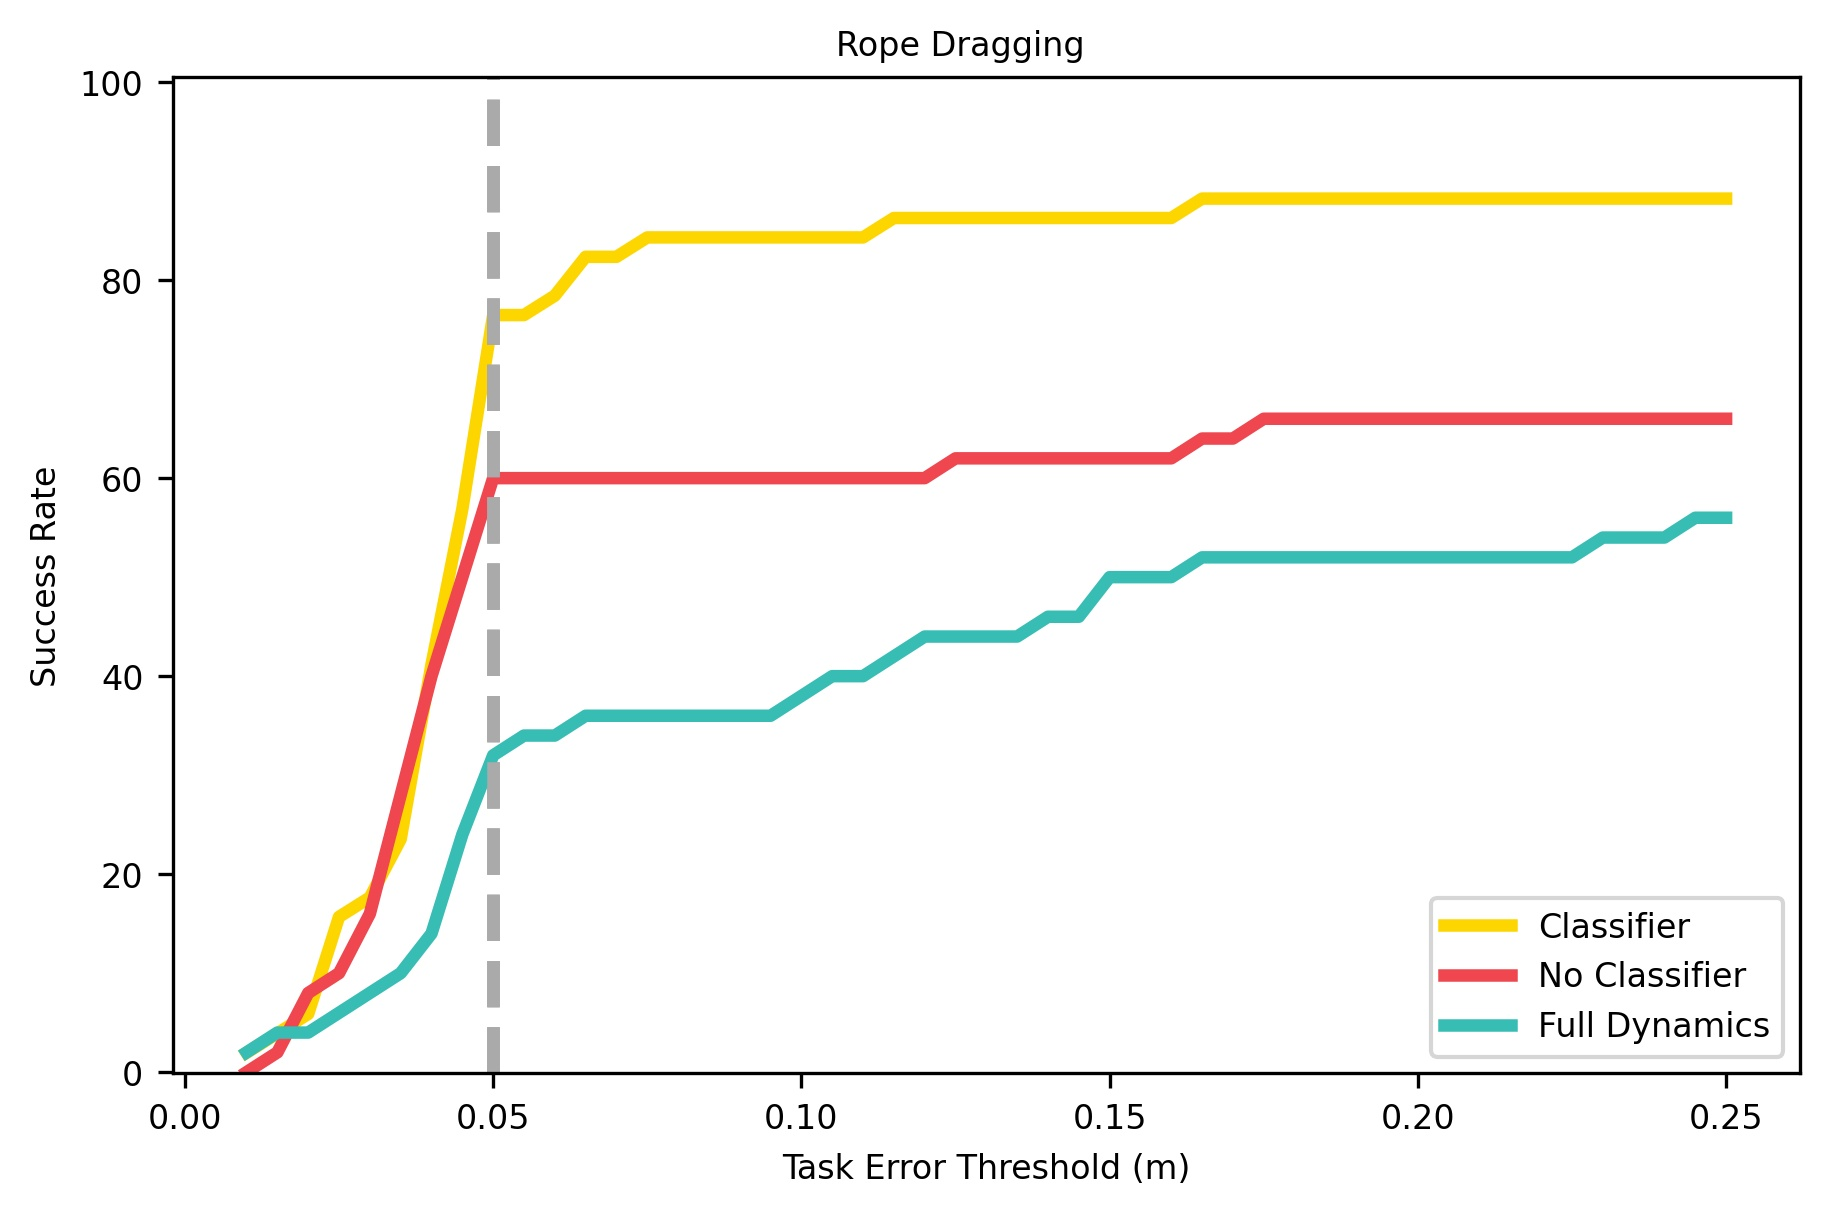
\includegraphics[width=\textwidth]{Chap2/images/dragging_success.jpeg}
        \label{Scirob:fig:dragging_success}
    \end{subfigure}
    \hfill
    \begin{subfigure}[b]{0.49\textwidth}
        \centering
        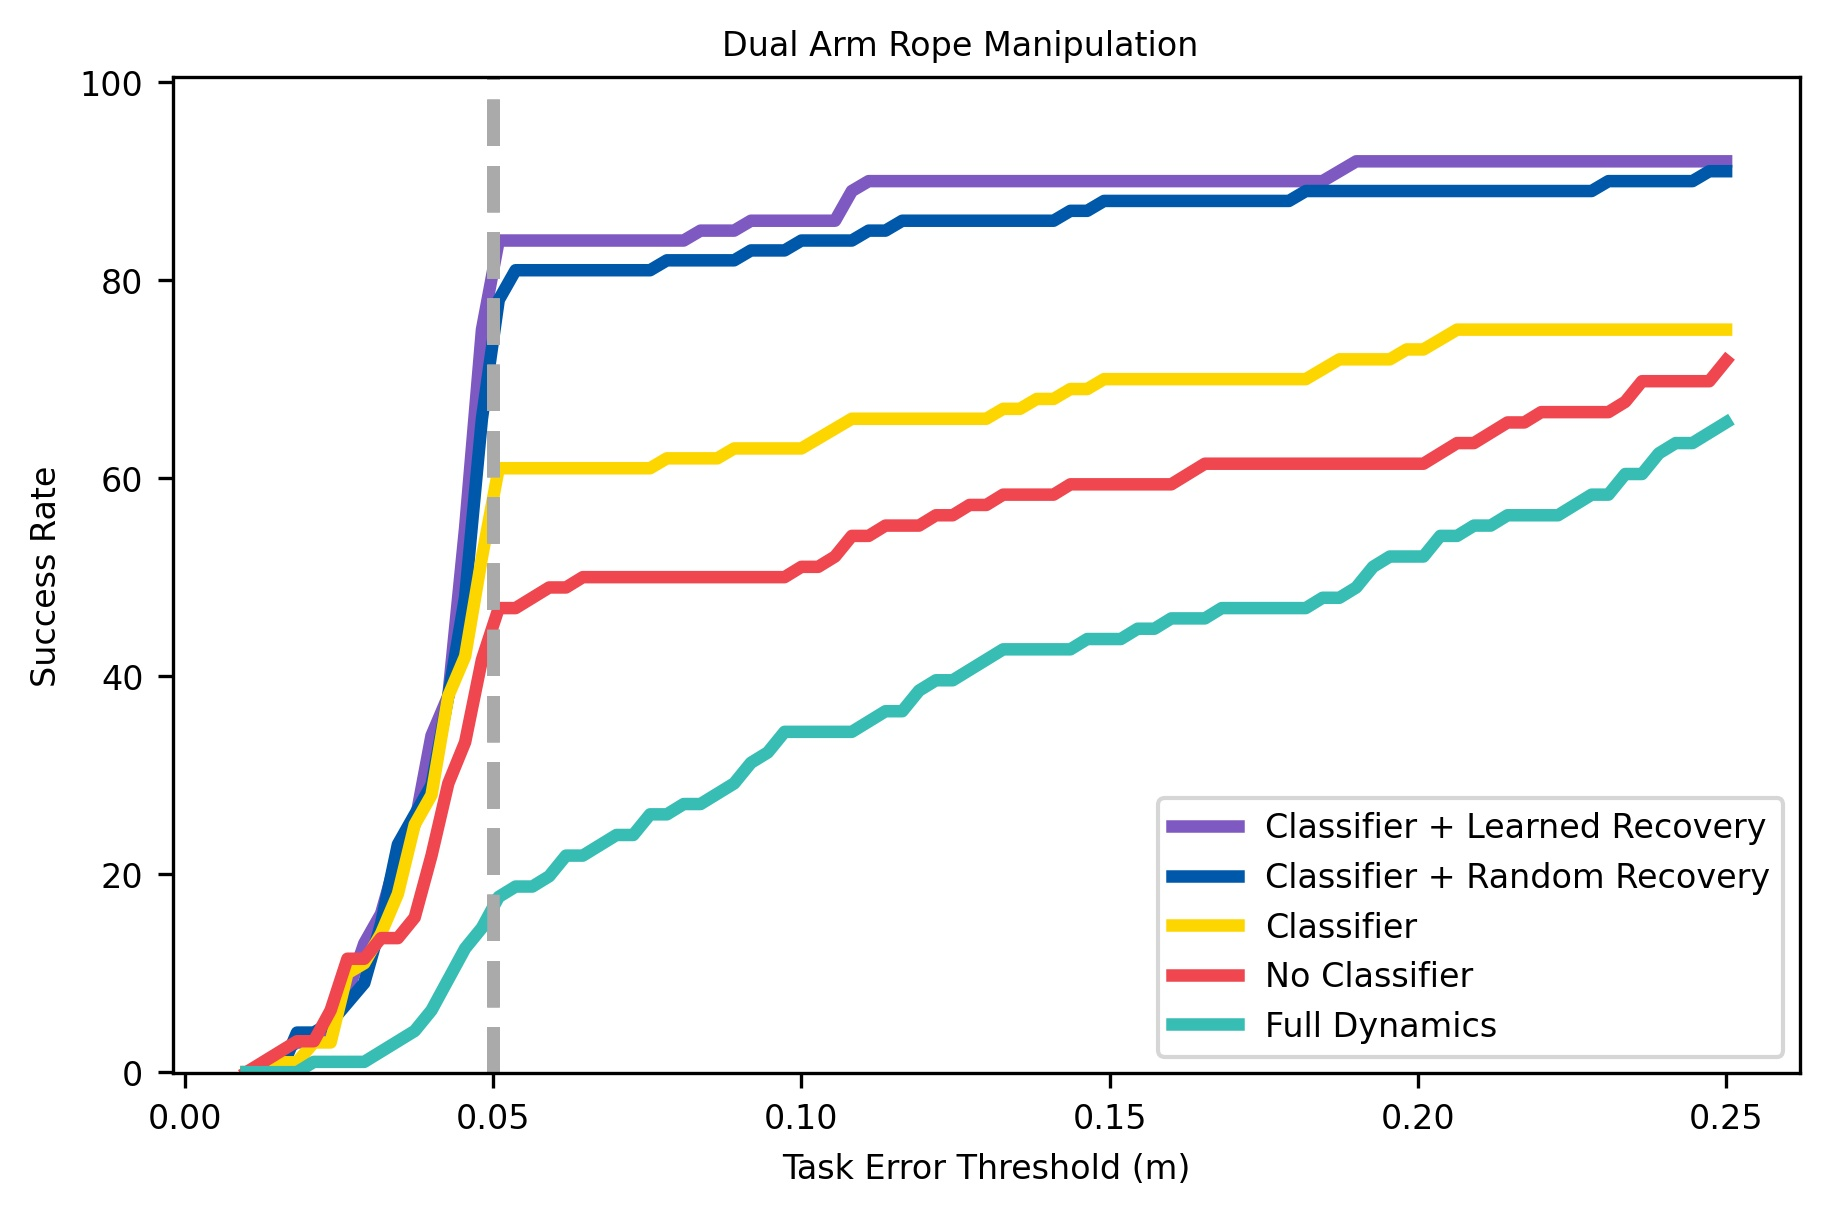
\includegraphics[width=\textwidth]{Chap2/images/dual_success.jpeg}
        \label{Scirob:fig:dual_success}
    \end{subfigure}
    \caption{Comparing success across methods. (left) The success rate as a function of the success threshold on task error for our simulated rope dragging experiments. The dashed line indicates the size of the goal region used. For example, this tells us that if our goal region was \SI{0.1}{\meter}, the "Classifier" method would achieve about 84\% success. (right) The success rate as a function of the success threshold on task error for our simulated dual arm rope manipulation experiments.}
    \label{Scirob:fig:figure6}
\end{figure}

Here we describe our results for using a robot for dual arm manipulation of rope among obstacles, as is shown in Figure \ref{Scirob:fig:figure2}b. Using two arms to manipulate deformable objects allows more control of the object than one arm and introduces additional interesting challenges in coordinating the two arms. The task we use for evaluation is to place the midpoint of the rope at a point in 3D while only holding the ends. In addition to obstacles, this scenario imposes the constraints of not overstretching the rope, not colliding the arms, and staying within the reachability limits of the robot. Task error is the Euclidean distance between the midpoint of the rope and the goal point. The goal region is defined as a sphere about the goal point with radius \SI{5}{\centi\meter}. This type of manipulation, while difficult for existing methods, is a prerequisite for many practical tasks such as cable harnessing.

The task error across 100 trials is shown in Figure \ref{Scirob:fig:figure6}b. Our complete method (\textit{Classifier + Learned Recovery}) reached the goal 84\% of the time with a mean task error of \SI{7.29}{\centi\meter}. This is statistically significantly (p $<0.001$) better than FD, which reached the goal 17.7\% of the time with a mean task error of \SI{20.32}{\centi\meter}, and No Classifier, which reached the goal 47\% of the time with a mean task error of \SI{16.97}{\centi\meter}. We also compare to our method without recovery actions, and to our method with random recovery actions. In this task, recovery actions are critical, and without them our method performs statistically significantly (p $<0.001$) worse with a success rate of 61\% and a mean task error of \SI{14.69}{\centi\meter}. When compared to random recovery actions, which reaches the goal 78\% of the time, our method has similar task error (p $= 0.281$ for the hypothesis that our method outperforms random recovery), however our method needs only a third as many recovery actions to achieve this task error. Over all 100 trials, random recovery used 613 recovery actions whereas our method used only 177. Additional numerical results are shown in Table \ref{Scirob:tab:dual_results}.

\subsection{Physical Robot Demonstrations}
We demonstrate potential applications of our method on real-world mock-ups of several domestic and automotive tasks. The first set of tasks are performed under the hood of a car, and require the robot to manipulate straps or hoses. These tasks include moving the midpoint of a hose to a specific location (Figure \ref{Scirob:fig:figure2}e), positioning the ends of a wiper fluid hose for installation (Figure \ref{Scirob:fig:figure2}f), and removing lifting straps from an engine (Figure \ref{Scirob:fig:figure2}d).

We also perform the task of fetching a charging cable (Figure \ref{Scirob:fig:figure2}c). In this example, the robot cannot reach the end of the cable directly because it is blocked by an obstacle. Instead, the robot grasps the cable elsewhere, and must drag the end of the cable towards the phone.

Notably, these tasks use several different types of goals described in the state space of the rope and grippers, all of which can be handled by our planner. This is in contrast to policy learning methods \cite{matas2018sim2real,Sundaresan2020,Wu2020} and methods which use goal images \cite{Nair2017,Finn2017,Zhang2019}. More details on how we perform these tasks can be found in Section ``\nameref{Scirob:sec:physical_robot_details}''.

\FloatBarrier

\begin{table}
    \centering
    \begin{tabular}{lllccccc}
    \hline\noalign{\smallskip}
     Name                        & Dynamics      & Classifier  & \makecell{max\\(m)} & \makecell{mean\\(m)} & \makecell{median\\(m)} & \makecell{std. dev.\\(m)} \\
    \noalign{\smallskip}\hline\hline\noalign{\smallskip}
     \makecell[l]{Classifier}    & Unconstrained & Learned     & 1.133   & 0.128    &  0.044     & 0.247 \\
     \noalign{\smallskip}\hline\noalign{\smallskip}
     \makecell[l]{No Classifier} & Unconstrained & None        & 1.408   & 0.325    &  0.045     & 0.425 \\
     \noalign{\smallskip}\hline\noalign{\smallskip}
     \makecell[l]{Full Dynamics} & Full          & None        & 1.519   & 0.438    &  0.156     & 0.450 \\
    \noalign{\smallskip}\hline
    \end{tabular}
    \caption{\label{Scirob:tab:dragging_results} Task error statistics for simulated rope dragging.}
\end{table}

\begin{table}
    \centering
    \begin{tabular}{lllccccc}
    \hline\noalign{\smallskip}
     Name                                        & Dynamics      & Classifier  & \makecell{max\\(m)} & \makecell{mean\\(m)} & \makecell{median\\(m)} & \makecell{std. dev.\\(m)} \\
    \noalign{\smallskip}\hline\hline\noalign{\smallskip}
     \makecell[l]{Classifier\\Learned\\Recovery} & Unconstrained & Learned    & 0.450   & 0.073    &  0.045     & 0.094 \\
     \noalign{\smallskip}\hline\noalign{\smallskip}
     \makecell[l]{Classifier\\Random\\Recovery}  & Unconstrained & Learned    & 0.629   & 0.081    &  0.046     & 0.106 \\
     \noalign{\smallskip}\hline\noalign{\smallskip}
     \makecell[l]{Classifier}                    & Unconstrained & Learned    & 0.630   & 0.147    &  0.047     & 0.167 \\
     \noalign{\smallskip}\hline\noalign{\smallskip}
     \makecell[l]{No Classifier}                 & Unconstrained & None       & 0.741   & 0.170    &  0.082     & 0.165 \\
     \noalign{\smallskip}\hline\noalign{\smallskip}
     \makecell[l]{Full Dynamics}                 & Full          & None       & 0.621   & 0.203    &  0.191     & 0.142 \\
    \noalign{\smallskip}\hline\noalign{\smallskip}
    \end{tabular}
    \caption{\label{Scirob:tab:dual_results}Task error statistics for simulated dual arm rope manipulation.}
\end{table}
\section{Conclusion}

In summary, the proposed method is able to complete a variety of difficult rope manipulation tasks in clutter. We are able to learn the unconstrained dynamics accurately, and by using our learned classifier, the planner successfully avoids the regions of state-action space where these unconstrained dynamics are incorrect. Using the classifier outperforms both using the full dynamics and simply trusting the unconstrained model by a wide margin. Last, recovery makes the method more resilient, allowing the robot to act even when it cannot trust its dynamics model. In our tabletop manipulation simulations, we demonstrated that these recovery actions statistically significantly improve the success rate of our method.